{
\begin{figure}
    \centering
    \begin{subfigure}[t]{0.4\textwidth}
        \centering
        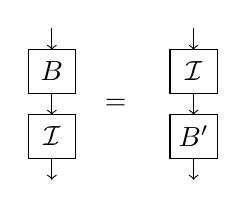
\begin{tikzpicture}[xscale=1.0, yscale=-0.55]
            \draw [->] (0,0) -- (0,0.5);
            \draw (-0.3,0.5) rectangle (0.3,1.5) node[pos=0.5] {$B$};
            \draw [->] (0,1.5) -- (0,2);
            \draw (-0.3,2) rectangle (0.3,3) node[pos=0.5] {$\mathcal{I}$};
            \draw [->] (0,3) -- (0,3.5);
            \draw (0.55,1.75) node[anchor=west] {$=$};
            \draw [->] (1.8,0) -- (1.8,0.5);
            \draw (1.5,0.5) rectangle (2.1,1.5) node[pos=0.5] {$\mathcal{I}$};
            \draw [->] (1.8,1.5) -- (1.8,2);
            \draw (1.5,2) rectangle (2.1,3) node[pos=0.5] {$B'$};
            \draw [->] (1.8,3) -- (1.8,3.5);
        \end{tikzpicture}
        \FigDef{propagation-affine-inverse-a}{Linear, $B(x)=\lambda x^{2^e}$}
    \end{subfigure}
    \hspace{0.3cm}
    \begin{subfigure}[t]{0.45\textwidth}
        \centering
        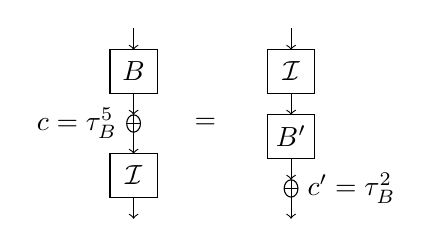
\begin{tikzpicture}[xscale=1.0, yscale=-0.55]
            \draw [->] (0,0) -- (0,0.5);
            \draw (-0.3,0.5) rectangle (0.3,1.5) node[pos=0.5] {$B$};
            \draw [->] (0,1.5) -- (0,2);
            \draw (0,2.2) ellipse (0.0875 and 0.2);
            \draw (0,2) -- (0,2.4);
            \draw (-0.0875,2.2) -- (0.0875,2.2);
            \draw (-0.0875,2.2) node[anchor=east] {$c=\tau_B^5$};
            \draw [->] (0,2.4) -- (0,2.9);
            \draw (-0.3,2.9) rectangle (0.3,3.9) node[pos=0.5] {$\mathcal{I}$};
            \draw [->] (0,3.9) -- (0,4.4);
            \draw (0.65,2.2) node[anchor=west] {$=$};
            \draw [->] (2,0) -- (2,0.5);
            \draw (1.7,0.5) rectangle (2.3,1.5) node[pos=0.5] {$\mathcal{I}$};
            \draw [->] (2,1.5) -- (2,2);
            \draw (1.7,2) rectangle (2.3,3) node[pos=0.5] {$B'$};
            \draw [->] (2,3) -- (2,3.5);
            \draw (2,3.7) ellipse (0.0875 and 0.2);
            \draw (2,3.5) -- (2,3.9);
            \draw (1.9125,3.7) -- (2.0875,3.7);
            \draw (2.0875,3.7) node[anchor=west] {$c'=\tau_B^2$};
            \draw [->] (2,3.9) -- (2,4.4);
        \end{tikzpicture}
        \FigDef{propagation-affine-inverse-b}{Affine, arbitrary $B\in\linbij{3}$}
    \end{subfigure}
    \FigDef{propagation-affine-inverse}{Propagation of linear/affine maps through the finite field inverse (only $\fielde{3}$).}
\end{figure}
}
